\chapter[Processo da Engenharia de Requisitos]{Processo da Engenharia de Requisitos}
O processo descrito a seguir foi modelado na ferramenta "Bizagi BPMN Modeler". Como dito anteriormente a abordagem a ser utilizada será uma abordagem ágil, fundamentada no SAFe(Scaled Agile Framework).

A estrutura dos três níveis do SAFe foi mantida porque, segundo Leffingwell(2011), ao ir baixando o nível de abstração dos requisitos mais gradativamente, é reduzido o nível de especificação precoce, reduzindo a sobrecarga ao gerenciar os requisitos. Isso também aumenta a agilidade do time por permitir a interpretação dos requisitos de maneira mais fácil para a implementação.(Leffingwell, 2011)
\section{Big picture do projeto}
  \begin{figure}[!htbp]
    \centering
    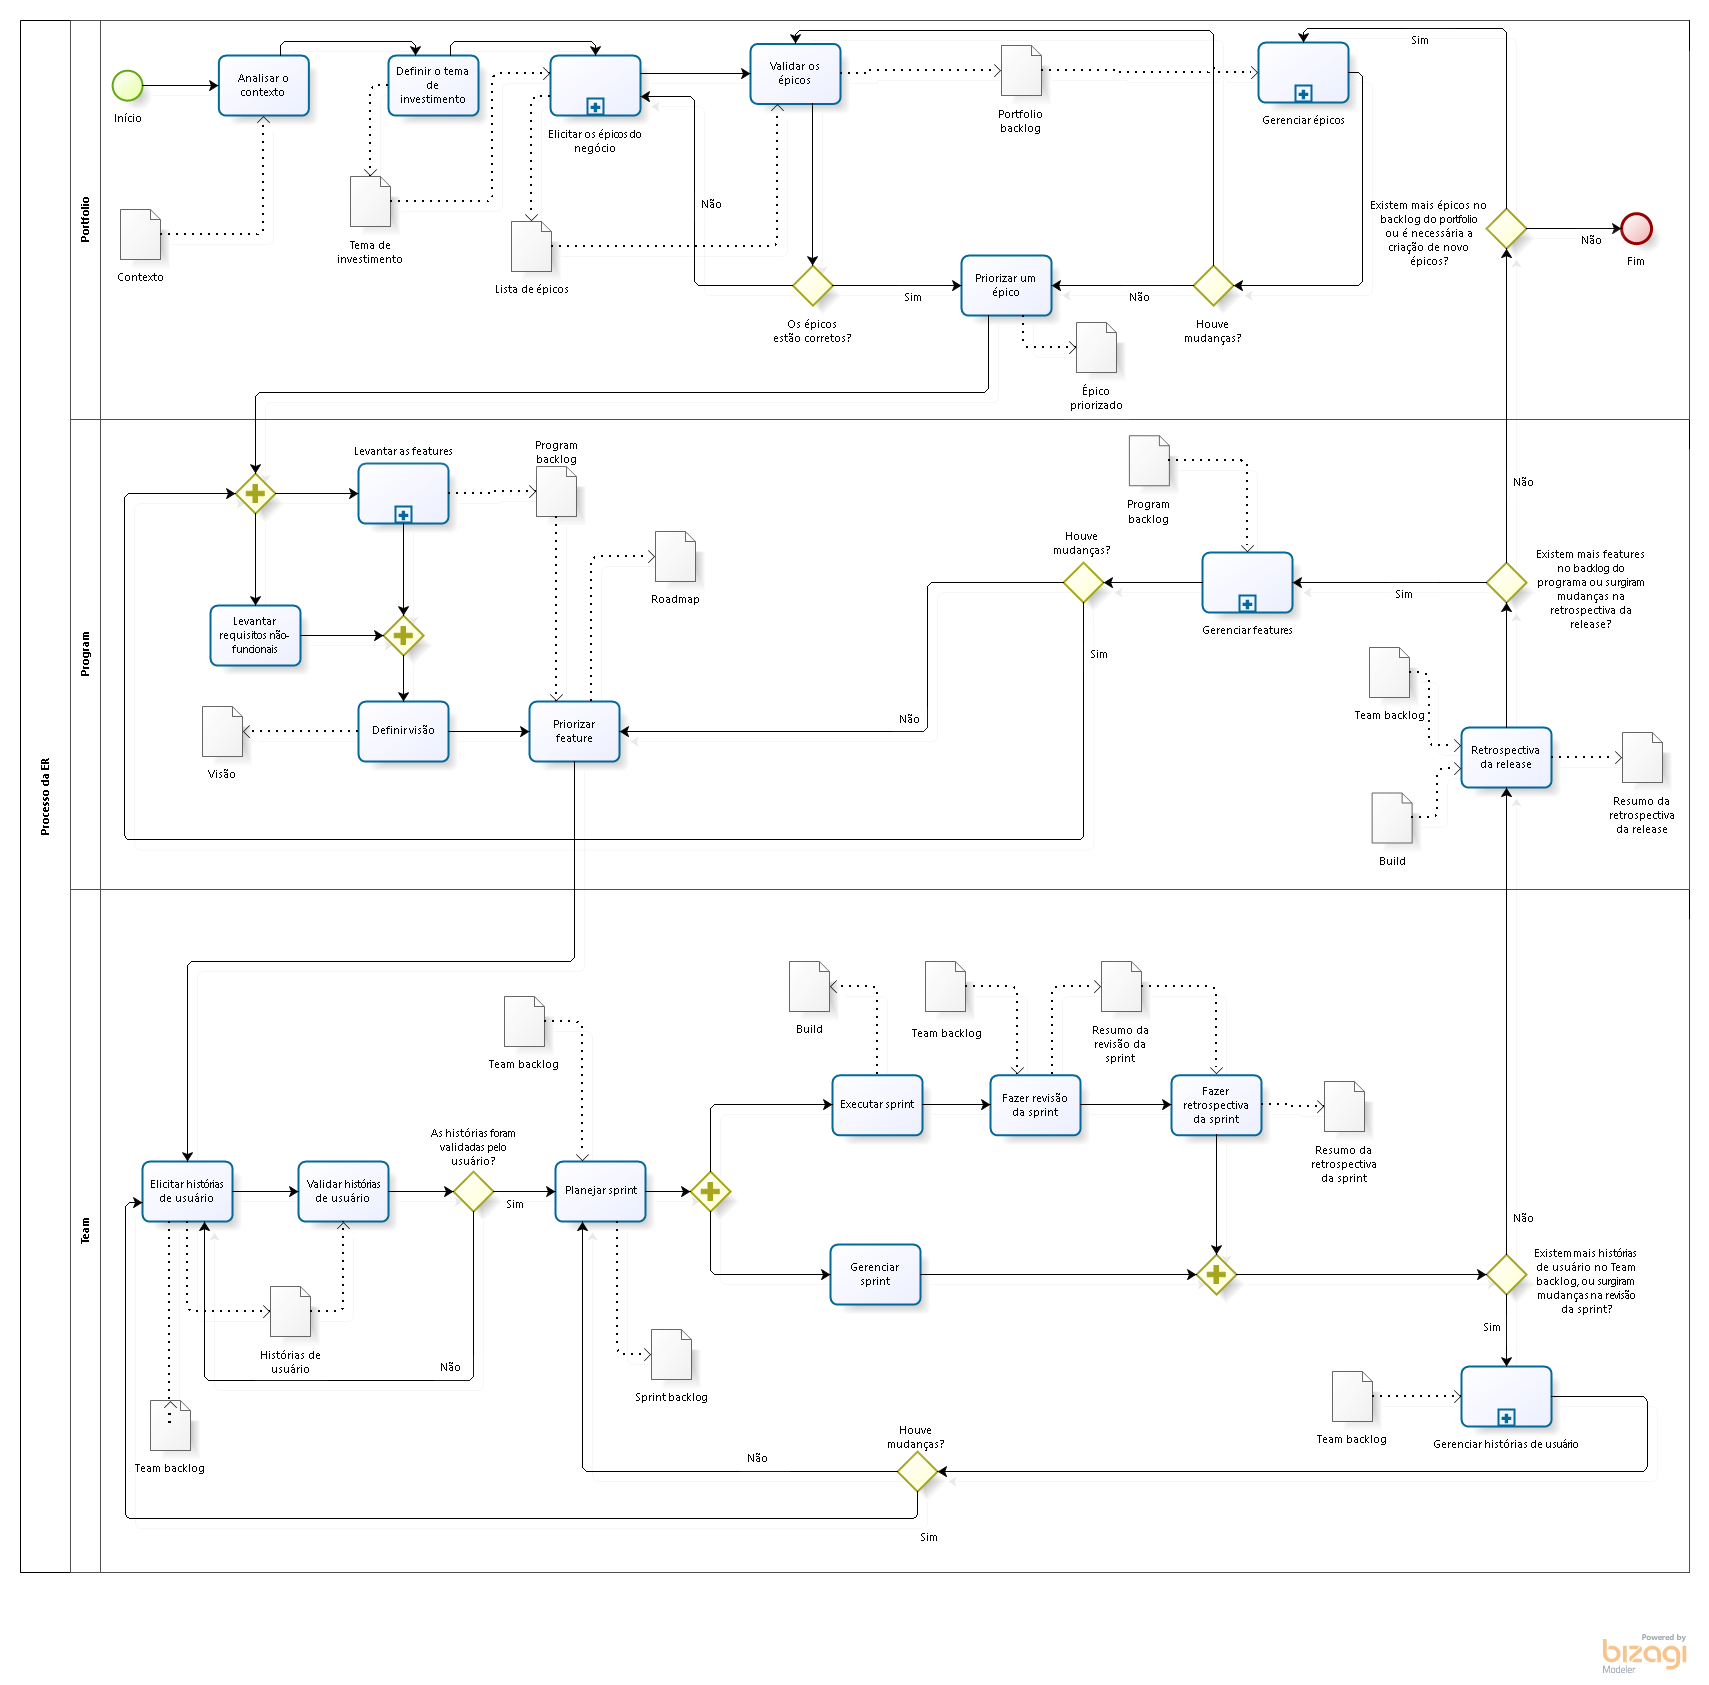
\includegraphics[scale=0.3]{figuras/Processo_v1-2}
    \caption[Big picture do processo.]{Big picture do processo. \footnotemark}
    \label{processo}
  \end{figure}
\section{Papéis no processo}
\textbf{Especialista do negócio} - É o \textit{stakeholder} que detém o conhecimento do negócio, do contexto organizacional e da visão do produto.

\textbf{Product owner} - É o membro do time que fica responsável pela definição das histórias e pela priorização do 
\textit{team backlog}, além de participar do planejamento e validação da sprint, definindo os seus objetivos.

\textbf{Product Manager} - De acordo com Leffingwell(2011), cabe ao PM: manter a visão e o program backlog, priorizar features, manter o roadmap, gerenciar o conteúdo da release e manter e priorizar o porfolio backlog. As atividades realizadas pelo PM acontecem nos níveis Portfolio e Program.

\textbf{Scrum Master} - O papel do Scrum Master é dar assistência para o resto da equipe, aplicando os príncipios da metodologia em questão, a fim de extrair máxima perfomance. Ele é, de certa forma, o líder do time. (Leffingwell, 2011)
\textbf{Time} - O time é composto por toda a equipe: desenvolvedores, designers e etc.
\section{Atividades e artefatos do processo}
\textbf{Temas de investimento} - Representam um conjunto de iniciativas guias para o investimento da instituição, seja em sistemas, produtos, aplicações ou serviços(Leffingwell, 2011).

\textbf{Épicos} - São iniciativas de desenvolvimento em larga escala que agregam valor a um tema de investimento(Leffingwell, 2011). São os de requisitos que possuem o mais alto nível no processo(Leffingwell, 2011).

\textbf{Portfolio backlog} - É o local onde os épicos são registrados, como um repositório de épicos.

\textbf{Features} - Atuam como pontes entre as necessidades dos stakeholders e os requisitos específicos no domínio da solução(Leffingwell, 2011).

\textbf{Program backlog} - É o local onde as features são registradas, como um repositório de features.

\textbf{Roadmap} - Consiste em uma série de releases com datas planejadas, cada uma pertinente a um tema, um conjunto de objetivos e uma feature priorizada. O roadmap nos dá uma ideia de como a instituição planeja mostrar valor com o decorrer do tempo(Leffingwell, 2011).

\textbf{Visão} - É um mecanismo utilizado para definir e comunicar a visão do sistema(Leffingwell, 2011). A visão de um sistema é composta por um conjunto de features que irão descrever as possibilidades do sistema, isto é, tudo aquilo que ele poderá oferecer ao usuário a fim de atender as necessidades dos envolvidos(Leffingwell, 2011).

\textbf{Team backlog} - Representa uma coleção de tudo que o time necessita para progredir aquela porção do sistema. Pode conter histórias de usuário ou enabler histories. Sendo que a maioria tem origem no program backlog, enquanto algumas são pertinentes a um contexto específico do time. O team backlog pertence ao PO, vale salientar que o fato de "pertencer" ao PO não significa que ele é o único que pode alterá-lo, mas é preferível que seja ele a fazer isso. (SAFe, 2015)

\textbf{Sprint backlog} - É o local onde serão armazenadas as histórias de usuário a serem realizadas naquela sprint.

\textbf{Build} - É o incremento de software gerado em cada sprint.